\chapter{El mar de Dirac, la masa de los fermiones y los espinores de cuatro componentes}

\section{Fermiones que se mueven hacia la derecha y el mar de Dirac}

La ecuación de Dirac es una ecuación para fermiones. Los bosones relativistas satisfacen ecuaciones distintas, como la ecuación de Klein--Gordon o las ecuaciones de Maxwell. El ejemplo más sencillo se da en una dimensión espacial y describe inicialmente partículas y antipartículas que solo pueden moverse hacia la derecha.

Partamos de una onda plana,
\begin{equation}
\psi(x,t)=\psi_0 e^{i(kx-\omega t)}.
\end{equation}
Su velocidad de fase es
\begin{equation}
v_{\mathrm{ph}}=\frac{\omega}{k}.
\end{equation}
Los signos de \(k\) y \(\omega\) son importantes. Si tienen el mismo signo, la fase se mueve hacia la derecha; si tienen signos opuestos, se mueve hacia la izquierda. Cuando \(\omega\) es proporcional a \(k\), las velocidades de fase y de grupo coinciden:
\begin{equation}
v_{\mathrm{g}}=\frac{d\omega}{dk}=\frac{\omega}{k}.
\end{equation}

Consideremos la ecuación de primer orden
\begin{equation}
\frac{\partial\psi}{\partial x}
+
\frac{\partial\psi}{\partial t}
=0.
\end{equation}
Al sustituir la onda plana se obtiene
\begin{equation}
ik\psi-i\omega\psi=0,
\end{equation}
y, por tanto,
\begin{equation}
\omega=k.
\end{equation}
Así pues, la onda se mueve hacia la derecha. Conviene etiquetar el campo en consecuencia:
\begin{equation}
\frac{\partial\psi_R}{\partial t}
=
-\frac{\partial\psi_R}{\partial x}.
\end{equation}

Al restituir la velocidad de la luz se obtiene la forma dimensional
\begin{equation}
\frac{\partial\psi_R}{\partial x}
+
\frac{1}{c}\frac{\partial\psi_R}{\partial t}
=0,
\end{equation}
de modo que
\begin{equation}
\omega=ck.
\end{equation}
A partir de ahora, \(c=1\). Con \(\hbar=1\), \(\omega\) también es la energía de un cuanto.

\begin{figure}[htbp]
\centering
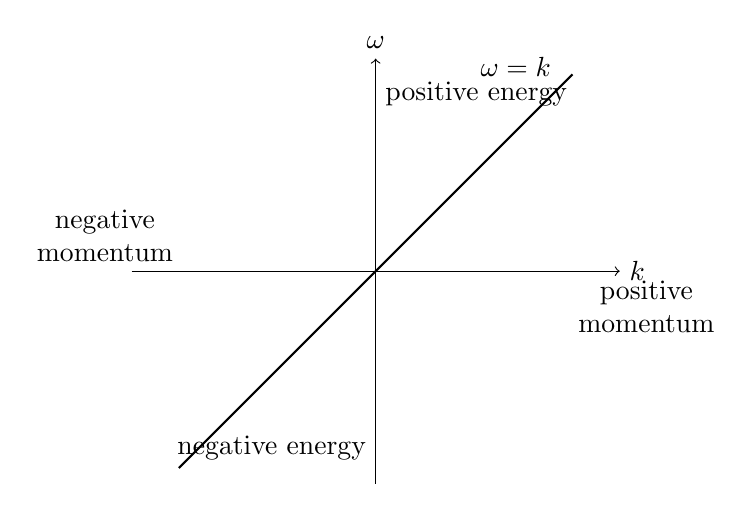
\begin{tikzpicture}[scale=1.0]
\draw[->] (-3.1,0) -- (3.1,0) node[right] {$k$};
\draw[->] (0,-2.7) -- (0,2.7) node[above] {$\omega$};
\draw[thick] (-2.5,-2.5) -- (2.5,2.5);
\node[above left] at (2.35,2.35) {$\omega=k$};
\node[below right,align=center] at (2.45,0) {positive\\momentum};
\node[above left,align=center] at (-2.45,0) {negative\\momentum};
\node[right] at (0,2.25) {positive energy};
\node[left] at (0,-2.25) {negative energy};
\end{tikzpicture}
\caption{La relación de dispersión sin masa para el movimiento hacia la derecha, \(\omega=k\), contiene ramas de energía positiva y negativa.}
\end{figure}

La recta tiene una consecuencia grave. Un valor positivo de \(k\) da energía positiva, mientras que un valor negativo de \(k\) da energía negativa. Sin embargo, ambas partes describen ondas que se mueven hacia la derecha, porque \(\omega/k=1\) en toda la recta.

Un electrón situado en la parte de energía positiva podría caer a un estado de menor energía, emitir un fotón de energía positiva, volver a caer y seguir recorriendo el espectro: un escalón hacia abajo, luego otro y otro más. Ningún electrón sería estable. Y, lo que es más grave, el mundo reduciría su energía produciendo cada vez más electrones de energía negativa.

La exclusión fermiónica aporta la solución. Llenemos todos los estados electrónicos de energía negativa. No puede entrar un segundo electrón en un estado ya ocupado, así que el sector de energía negativa completamente lleno impide una caída ilimitada. Este sector lleno es el mar de Dirac, y su estado completamente lleno es el estado fundamental, o vacío.

\begin{classroomqa}
\lecturetimestamp{00:07:19}
\audiencequestion{¿Hay infinitos estados de energía negativa cada vez menores?}
\lecturerresponse{Sí. Con momentos discretos, el espectro se parece a una escalera infinita; con momentos continuos, a una pendiente continua. Llenar el mar de energía negativa impide que un electrón descienda indefinidamente, aunque aún puede producirse una transición finita hacia abajo con emisión de un fotón si hay disponible un estado inferior desocupado.}
\end{classroomqa}

Esto explica por qué una ecuación con este espectro debe cuantizarse como una teoría fermiónica. Si los cuantos fueran bosones, podría haber un número arbitrario de ellos en el mismo estado inferior, y llenar el sector de energía negativa no estabilizaría el vacío.

La imagen del mar lleno también da lugar a las antipartículas. En el vacío, todos los niveles de energía negativa están ocupados y todos los de energía positiva están vacíos. Un electrón puede pasar de cualquier nivel ocupado de energía negativa a cualquier nivel desocupado de energía positiva; no es necesario que los niveles inicial y final estén situados simétricamente.

\begin{figure}[htbp]
\centering
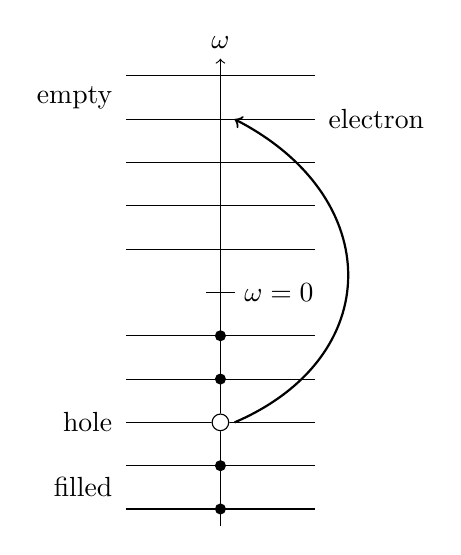
\begin{tikzpicture}[x=1cm,y=0.55cm]
\draw[->] (0,-5.4) -- (0,5.4) node[above] {$\omega$};
\draw (-0.18,0) -- (0.18,0) node[right] {$\omega=0$};
\foreach \y in {-5,-4,-3,-2,-1} {
  \draw (-1.2,\y) -- (1.2,\y);
  \fill (0,\y) circle (2pt);
}
\foreach \y in {1,2,3,4,5} {
  \draw (-1.2,\y) -- (1.2,\y);
}
\draw[->,thick] (0.18,-3) .. controls (2.1,-1.5) and (2.1,2.2) .. (0.18,4);
\draw[white,fill=white] (0,-3) circle (3pt);
\draw (0,-3) circle (3pt);
\node[left] at (-1.25,-3) {hole};
\node[left] at (-1.25,-4.5) {filled};
\node[left] at (-1.25,4.5) {empty};
\node[right] at (1.25,4) {electron};
\end{tikzpicture}
\caption{Al promover un electrón ocupado de energía negativa, se obtiene un electrón de energía positiva y queda un hueco en el mar lleno.}
\end{figure}

Quitar un electrón de energía negativa aumenta la energía con respecto al vacío, así que el hueco tiene energía positiva. En la rama \(\omega=k\), el electrón eliminado también tenía momento negativo. Al quitar un momento negativo queda un exceso positivo de momento, de modo que el hueco tiene momento positivo. Si se toma negativa la carga del electrón, el electrón que falta tiene carga positiva. Así, el hueco es una antipartícula de energía y momento positivos, mientras que el electrón promovido tiene carga negativa, energía positiva y momento positivo. Toda excitación real de esta teoría de una sola rama se mueve hacia la derecha.

El campo \(\psi_R\) se construye con operadores fermiónicos de creación y aniquilación. Por tanto, la interpretación en términos de partículas y huecos se refiere a los cuantos que el campo crea y elimina, y no solo a una onda clásica.

Aún hay una asimetría. El mar que se mueve hacia la derecha contiene estados de energía negativa con momento negativo. Su momento total formal es enorme y apunta hacia la izquierda. Se puede definir como cero el momento del vacío restando esa constante, pero el estado sigue desequilibrado en su estructura: las partículas y antipartículas solo se mueven hacia la derecha, mientras que el vacío lleno está formado por estados de momento negativo.

\section{La rama que se mueve hacia la izquierda y un vacío equilibrado}

Para equilibrar izquierda y derecha hace falta un segundo campo independiente, con sus propios operadores de creación y aniquilación. Supongamos que satisface
\begin{equation}
\frac{\partial\psi_L}{\partial t}
=
+\frac{\partial\psi_L}{\partial x}.
\end{equation}
Para la misma forma de onda plana,
\begin{equation}
-i\omega\psi_L=ik\psi_L,
\end{equation}
por lo que
\begin{equation}
\omega=-k.
\end{equation}
Esta segunda recta es la imagen especular de \(\omega=k\). Su rama de energía positiva describe partículas que se mueven hacia la izquierda, y también hay que llenar su rama de energía negativa.

\begin{figure}[htbp]
\centering
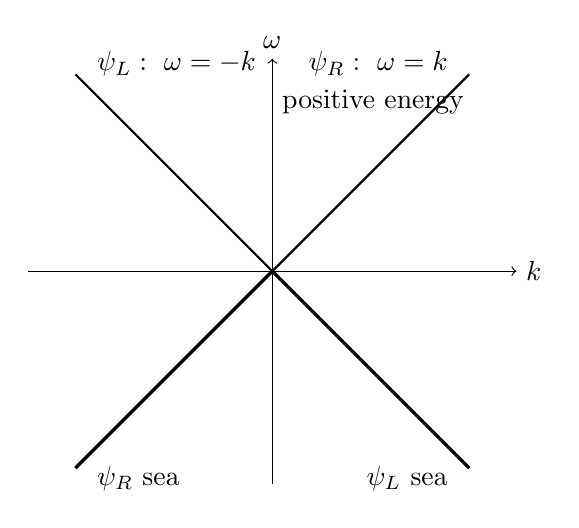
\begin{tikzpicture}[scale=1.0]
\draw[->] (-3.1,0) -- (3.1,0) node[right] {$k$};
\draw[->] (0,-2.7) -- (0,2.7) node[above] {$\omega$};
\draw[thick] (-2.5,-2.5) -- (2.5,2.5);
\draw[thick] (-2.5,2.5) -- (2.5,-2.5);
\draw[very thick] (-2.5,-2.5) -- (0,0);
\draw[very thick] (0,0) -- (2.5,-2.5);
\node[above left] at (2.35,2.35) {$\psi_R:\ \omega=k$};
\node[above right] at (-2.35,2.35) {$\psi_L:\ \omega=-k$};
\node[right] at (0,2.15) {positive energy};
\node[below right] at (-2.35,-2.35) {$\psi_R$ sea};
\node[below left] at (2.35,-2.35) {$\psi_L$ sea};
\end{tikzpicture}
\caption{Los campos independientes que se mueven hacia la derecha y hacia la izquierda dan lugar a ramas sin masa reflejadas; en el vacío se llenan las dos semirramas de energía negativa.}
\end{figure}

Tras llenar ambos mares de energía negativa, hay tantos estados ocupados que se mueven hacia la izquierda como hacia la derecha. Sus momentos se compensan en el vacío. Las excitaciones de partículas y huecos pueden moverse ahora en cualquiera de las dos direcciones.

\begin{classroomqa}
\lecturetimestamp{00:15:58}
\audiencequestion{¿Se puede resolver el problema de la energía negativa sin postular estados llenos y huecos?}
\lecturerresponse{Se puede volver a etiquetar la misma teoría. Un estado electrónico lleno de energía negativa puede llamarse estado vacío de una antipartícula; así, el lenguaje físico solo incluye partículas y antipartículas de energía positiva. La imagen del mar lleno sigue siendo una comprobación útil de coherencia, como la de una banda llena en un metal: al quitar un electrón se produce un hueco, mientras que al promoverlo se producen una partícula y un hueco.}
\end{classroomqa}

Las excitaciones consideradas hasta aquí no tienen masa. Sus relaciones de dispersión son lineales y sus velocidades tienen módulo \(1\), así que se mueven a la velocidad de la luz. La siguiente pregunta es cómo dotarlas de masa.

\section{Dos componentes y el término de masa}

Primero, reunamos los dos campos en una columna:
\begin{equation}
\Psi=
\begin{pmatrix}
\psi_R\\
\psi_L
\end{pmatrix}.
\end{equation}
Por ahora, esto no es más que una notación compacta para dos ecuaciones independientes. Definamos
\begin{equation}
\alpha=
\begin{pmatrix}
1&0\\
0&-1
\end{pmatrix}.
\end{equation}
Entonces, las ecuaciones para los campos que se mueven hacia la derecha y hacia la izquierda quedan
\begin{equation}
\frac{\partial\Psi}{\partial t}
=
-\alpha\frac{\partial\Psi}{\partial x}.
\end{equation}

\begin{figure}[htbp]
\centering
\includegraphics[width=0.78\textwidth]{lecture_06_figure_02.png}
\caption{Los campos \(\psi_R\) y \(\psi_L\) forman un espinor de dos componentes; \(\alpha\) distingue las dos ramas sin masa.}
\lectureframe{00:20:36}
\end{figure}

Para una onda plana, los operadores
\begin{equation}
i\partial_t
\quad\hbox{and}\quad
-i\partial_x
\end{equation}
devuelven \(\omega\) y \(k\), respectivamente. Por tanto, la ecuación matricial puede abreviarse así:
\begin{equation}
\omega=\alpha k.
\end{equation}
Para la componente superior, esto significa \(\omega=k\); para la inferior, significa \(\omega=-k\). La notación ha condensado las dos ecuaciones, pero no ha introducido nueva física.

Los electrones no carecen de masa ni se mueven a la velocidad de la luz. Una fórmula tentadora para su energía es la energía cinética no relativista \(k^2/(2m)\), pero no puede ser el punto de partida aquí: el límite sin masa ya describe un movimiento a la velocidad de la luz. La relación relativista es
\begin{equation}
\omega^2=k^2+m^2,
\end{equation}
o, si incluimos ambas ramas de energía,
\begin{equation}
\omega=\pm\sqrt{k^2+m^2}.
\end{equation}
Cuando \(m=0\), estas se reducen a \(\omega=k\) y \(\omega=-k\).

\begin{classroomqa}
\lecturetimestamp{00:25:23}
\audiencequestion{¿Se están usando unidades en las que \(c=1\) y cómo se obtiene la velocidad de una partícula masiva?}
\lecturerresponse{Sí. La velocidad de un paquete de ondas es la velocidad de grupo, \(v_{\mathrm g}=d\omega/dk=k/\sqrt{k^2+m^2}\), en la rama de energía positiva. Así, la propia relación de dispersión incluye la reducción de la velocidad por debajo de \(c=1\) para una partícula masiva.}
\end{classroomqa}

\begin{classroomqa}
\lecturetimestamp{00:26:29}
\audiencequestion{En la notación abreviada \(\omega=\alpha k\), ¿\(\omega\) es un vector o una matriz?}
\lecturerresponse{La notación abreviada representa una ecuación de operadores que actúa sobre la función de onda de dos componentes. Aquí, \(\omega\) significa \(i\partial_t\), \(k\) significa \(-i\partial_x\) y \(\alpha\) es la matriz que actúa sobre el índice de componente. Los símbolos escalares \(\omega\) y \(k\) solo pasan a ser sus valores propios numéricos para una onda plana.}
\end{classroomqa}

Mantengamos la ecuación de primer orden y probemos la extensión más sencilla que depende de la masa:
\begin{equation}
\omega=\alpha k+\beta m.
\end{equation}
El objeto \(\beta\) debe ser una matriz, porque actúa sobre el mismo campo de dos componentes que \(\alpha\). Su álgebra se obtiene elevando al cuadrado:
\begin{align}
\omega^2
&=(\alpha k+\beta m)(\alpha k+\beta m)\\
&=\alpha^2k^2+\beta^2m^2
+\alpha\beta\,km+\beta\alpha\,mk\\
&=\alpha^2k^2+\beta^2m^2
+(\alpha\beta+\beta\alpha)km.
\end{align}
Para obtener \(k^2+m^2\) para cualquier \(k\) y \(m\), exigimos que
\begin{equation}
\alpha^2=I,
\qquad
\beta^2=I,
\qquad
\alpha\beta+\beta\alpha=0.
\end{equation}

Dos números ordinarios distintos de cero no pueden satisfacer la última condición: para números daría \(2\alpha\beta=0\), en contradicción con que ambos cuadrados sean \(1\). Las matrices sí pueden anticonmutar. En particular, \(\beta\) no puede ser igual a \(\alpha\), ya que entonces
\begin{equation}
\alpha\beta+\beta\alpha=2\alpha^2=2I.
\end{equation}

Elijamos
\begin{equation}
\beta=
\begin{pmatrix}
0&1\\
1&0
\end{pmatrix}.
\end{equation}
Su cuadrado se puede comprobar entrada por entrada:
\begin{equation}
\begin{aligned}
\beta^2
&=
\begin{pmatrix}
0&1\\
1&0
\end{pmatrix}
\begin{pmatrix}
0&1\\
1&0
\end{pmatrix}\\
&=
\begin{pmatrix}
0\cdot0+1\cdot1&0\cdot1+1\cdot0\\
1\cdot0+0\cdot1&1\cdot1+0\cdot0
\end{pmatrix}
=
\begin{pmatrix}
1&0\\
0&1
\end{pmatrix}.
\end{aligned}
\end{equation}
El orden de la multiplicación importa:
\begin{align}
\alpha\beta
&=
\begin{pmatrix}
1&0\\
0&-1
\end{pmatrix}
\begin{pmatrix}
0&1\\
1&0
\end{pmatrix}
=
\begin{pmatrix}
0&1\\
-1&0
\end{pmatrix},\\
\beta\alpha
&=
\begin{pmatrix}
0&1\\
1&0
\end{pmatrix}
\begin{pmatrix}
1&0\\
0&-1
\end{pmatrix}
=
\begin{pmatrix}
0&-1\\
1&0
\end{pmatrix}.
\end{align}
Por tanto,
\begin{equation}
\alpha\beta=-\beta\alpha,
\qquad
\alpha\beta+\beta\alpha=0.
\end{equation}
Hay otras elecciones de matrices equivalentes, pero esta hace especialmente claras las ecuaciones para las componentes.

Al restituir los operadores diferenciales se obtiene la ecuación con masa
\begin{equation}
i\frac{\partial\Psi}{\partial t}
=
-i\alpha\frac{\partial\Psi}{\partial x}
+m\beta\Psi.
\end{equation}
La matriz \(\beta\) intercambia las componentes:
\begin{equation}
\beta
\begin{pmatrix}
\psi_R\\
\psi_L
\end{pmatrix}
=
\begin{pmatrix}
\psi_L\\
\psi_R
\end{pmatrix}.
\end{equation}
En consecuencia,
\begin{align}
i\dot{\psi}_R
&=-i\frac{\partial\psi_R}{\partial x}+m\psi_L,\\
i\dot{\psi}_L
&=+i\frac{\partial\psi_L}{\partial x}+m\psi_R.
\end{align}

El término de masa acopla campos que eran independientes en la teoría sin masa. La ecuación de la componente superior contiene la componente inferior, y la ecuación de la componente inferior contiene la superior. A esto se refiere la masa de Dirac. Las ecuaciones son invariantes bajo traslaciones, por lo que conservan el momento, y la masa de las excitaciones de partículas que describen es \(m\).

\begin{classroomqa}
\lecturetimestamp{00:38:25}
\audiencequestion{¿Una solución es automáticamente invariante de Lorentz?}
\lecturerresponse{Una solución particular no debería permanecer inalterada bajo una transformación de Lorentz. Un estado con un momento dado se transforma en un estado con el momento transformado, así que lo que corresponde exigir es covariancia. La relación \(\omega^2=k^2+m^2\) es una comprobación clave de invariancia de Lorentz, pero la covariancia completa también requiere conocer la ley de transformación del espinor \(\Psi\), que aún no se ha establecido.}
\end{classroomqa}

\section{El sistema en reposo y el significado de las componentes}

No se puede llevar al reposo una partícula sin masa, pero sí una partícula masiva. En reposo, \(k=0\), así que la función de onda no varía en el espacio y
\begin{equation}
\omega=\beta m.
\end{equation}
La ecuación diferencial se reduce a
\begin{equation}
i\frac{d\Psi}{dt}=m\beta\Psi.
\end{equation}
En componentes,
\begin{align}
i\dot{\psi}_R&=m\psi_L,\\
i\dot{\psi}_L&=m\psi_R.
\end{align}
Las dos entradas no diagonales de \(\beta\) son \(+1\), así que ninguna de estas ecuaciones lleva un signo menos adicional.

Las ecuaciones se desacoplan al sumar y restar las componentes. Definamos
\begin{equation}
\psi_+=\psi_R+\psi_L,
\qquad
\psi_-=\psi_R-\psi_L.
\end{equation}
Al sumar las dos ecuaciones en el sistema en reposo se obtiene
\begin{equation}
i\dot{\psi}_+=m\psi_+,
\end{equation}
mientras que al restarlas se obtiene
\begin{equation}
i\dot{\psi}_-=-m\psi_-.
\end{equation}
Por tanto,
\begin{equation}
\omega=+m
\quad\hbox{for }\psi_+,
\qquad
\omega=-m
\quad\hbox{for }\psi_-.
\end{equation}

\begin{figure}[htbp]
\centering
\includegraphics[width=0.62\textwidth]{lecture_06_figure_03.png}
\caption{Con momento nulo, \(\psi_+=\psi_R+\psi_L\) y \(\psi_-=\psi_R-\psi_L\) tienen frecuencias de reposo \(\omega=+m\) y \(\omega=-m\).}
\lectureframe{00:44:49}
\end{figure}

El campo en reposo de energía positiva es \(\psi_+\); el campo en reposo de energía negativa es \(\psi_-\). Los estados de energía negativa se llenan, como antes. El resultado en el sistema en reposo corresponde solo al corte \(k=0\) del espectro completo:
\begin{equation}
\omega_\pm(k)=\pm\sqrt{k^2+m^2}.
\end{equation}
\begin{figure}[htbp]
\centering
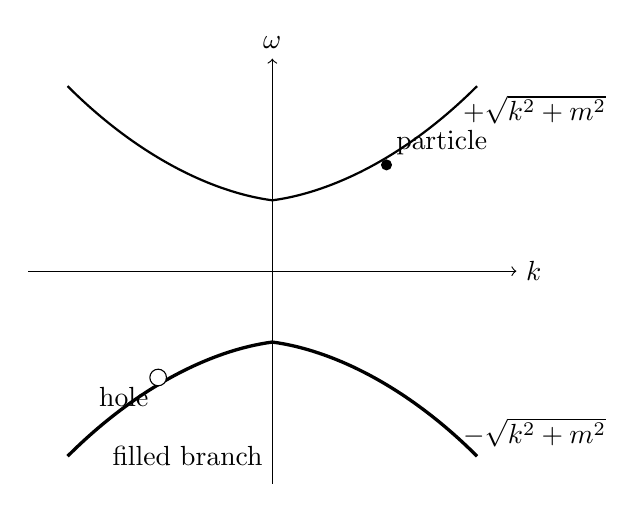
\begin{tikzpicture}[scale=1.0]
\draw[->] (-3.1,0) -- (3.1,0) node[right] {$k$};
\draw[->] (0,-2.7) -- (0,2.7) node[above] {$\omega$};
\draw[thick] (-2.6,2.35)
  .. controls (-1.7,1.45) and (-0.75,1.0) .. (0,0.9)
  .. controls (0.75,1.0) and (1.7,1.45) .. (2.6,2.35);
\draw[very thick] (-2.6,-2.35)
  .. controls (-1.7,-1.45) and (-0.75,-1.0) .. (0,-0.9)
  .. controls (0.75,-1.0) and (1.7,-1.45) .. (2.6,-2.35);
\fill (1.45,1.35) circle (2pt);
\node[above right] at (1.45,1.35) {particle};
\fill[white] (-1.45,-1.35) circle (3pt);
\draw (-1.45,-1.35) circle (3pt);
\node[below left] at (-1.45,-1.35) {hole};
\node[right] at (2.3,2.05) {$+\sqrt{k^2+m^2}$};
\node[right] at (2.3,-2.05) {$-\sqrt{k^2+m^2}$};
\node[left] at (0,-2.35) {filled branch};
\end{tikzpicture}
\caption{Para cada momento, el espectro masivo tiene estados de energía positiva y negativa. La rama negativa está llena, y un estado ausente en ella es un hueco de energía positiva.}
\end{figure}
Para cada momento hay un estado de energía positiva y otro de energía negativa. Al llenar todos los estados de la rama negativa, quedan partículas de energía positiva por encima del mar y huecos de energía positiva en él. Tanto las partículas como los huecos tienen masa positiva.

Conviene repetir la idea esencial. Un fermión adquiere masa cuando se acoplan sus dos componentes, que antes eran independientes. En reposo, ninguna de las componentes originales por sí sola es un estado propio de la energía. Los estados de energía definida son la suma y la diferencia de ambas.

Para ver qué significa la suma, escribamos \(C_R^\dagger\) y \(C_L^\dagger\) para las partes pertinentes de creación de una partícula. Al actuar sobre el vacío,
\begin{equation}
(C_R^\dagger+C_L^\dagger)\lvert0\rangle
\end{equation}
crea una partícula en una superposición coherente de las dos componentes. No crea dos partículas. Un producto,
\begin{equation}
C_R^\dagger C_L^\dagger\lvert0\rangle,
\end{equation}
contiene dos operadores de creación y crea un estado de dos partículas cuando ambos modos están disponibles. Tras normalizar el estado en reposo, las dos componentes tienen la misma probabilidad, pero la onda acoplada en su conjunto tiene momento nulo.

Las etiquetas \(R\) y \(L\) solo indicaban movimiento literal cuando \(m=0\). Una vez presente el término de masa, una solución masiva en movimiento suele contener ambas componentes, y la solución en reposo las contiene con igual magnitud. Por ello, aquí es preferible interpretar \(R\) y \(L\) como etiquetas de las componentes superior e inferior del espinor.

\begin{figure}[htbp]
\centering
\includegraphics[width=0.78\textwidth]{lecture_06_figure_04.png}
\caption{Para masa distinta de cero, las dos componentes del espinor están acopladas; su interpretación como componentes que se mueven hacia la derecha y hacia la izquierda solo se aplica directamente en el límite sin masa.}
\lectureframe{00:50:48}
\end{figure}

Todos los fermiones masivos de la física de partículas se construyen a partir de campos de componentes izquierdas y derechas: una masa de Dirac acopla componentes que son independientes en el límite sin masa.

\begin{classroomqa}
\lecturetimestamp{00:52:01}
\audiencequestion{¿Debe incluirse en \(\psi_R\pm\psi_L\) un factor de \(1/\sqrt{2}\)?}
\lecturerresponse{Se puede incluir para normalizar el estado. Multiplica ambos lados de la ecuación y, por tanto, no cambia la ecuación de movimiento.}
\end{classroomqa}

\begin{classroomqa}
\lecturetimestamp{00:52:12}
\audiencequestion{¿Importan las magnitudes relativas de las componentes derecha e izquierda?}
\lecturerresponse{Para los estados propios elegidos en el sistema en reposo, sus magnitudes son iguales. La normalización global es arbitraria, pero las magnitudes relativas quedan fijadas por el vector propio de \(\beta\).}
\end{classroomqa}

\begin{classroomqa}
\lecturetimestamp{00:52:52}
\audiencequestion{¿Podrían tener las dos componentes una fase relativa?}
\lecturerresponse{Sí. Los coeficientes reales de \(\psi_R\pm\psi_L\) se deben a que se ha elegido una matriz \(\beta\) real. Otras matrices que se elevan al cuadrado para dar la identidad y anticonmutan con \(\alpha\) son opciones equivalentes, y en ese caso pueden aparecer fases relativas entre las componentes. Una vez elegida una representación, hay que usarla de manera coherente.}
\end{classroomqa}

\begin{classroomqa}
\lecturetimestamp{00:53:43}
\audiencequestion{¿Son algo engañosas las etiquetas ``izquierdo'' y ``derecho'' después de añadir la masa?}
\lecturerresponse{En cierta medida. Describen ondas genuinamente dirigidas hacia la izquierda y hacia la derecha en la teoría sin masa. Con masa distinta de cero, incluso una partícula que se mueve en una sola dirección suele contener ambas componentes, así que son más precisas las etiquetas ``componente superior'' y ``componente inferior''.}
\end{classroomqa}

\begin{classroomqa}
\lecturetimestamp{00:55:01}
\audiencequestion{¿Una partícula fermiónica en reposo requiere ya momento angular de espín?}
\lecturerresponse{No en este modelo unidimensional. En una dimensión espacial no está definido el momento angular, así que el espín aún no forma parte de la construcción.}
\end{classroomqa}

\begin{classroomqa}
\lecturetimestamp{00:55:24}
\audiencequestion{¿La función de onda contiene operadores fermiónicos de creación y aniquilación?}
\lecturerresponse{Sí.}
\end{classroomqa}

\begin{classroomqa}
\lecturetimestamp{00:55:30}
\audiencequestion{Aparte de la elección de los operadores de creación y aniquilación, ¿dónde entra el carácter fermiónico?}
\lecturerresponse{Entra mediante las reglas fermiónicas de creación--aniquilación. Una ecuación con este espectro de energía negativa debe cuantizarse con esas reglas; las reglas de ocupación bosónicas dejarían inestable el vacío. Los bosones relativistas deben describirse mediante otra ecuación de onda.}
\end{classroomqa}

\begin{classroomqa}
\lecturetimestamp{00:56:20}
\audiencequestion{¿Se puede transformar mediante una transformación de Lorentz una solución con momento distinto de cero para obtener la solución en reposo?}
\lecturerresponse{Sí. Un impulso puede llevar una solución masiva a su sistema en reposo, pero para realizar la transformación hay que saber cómo actúan las transformaciones de Lorentz sobre el espinor \(\Psi\).}
\end{classroomqa}

\section{La masa a partir de un campo escalar en el vacío}

\begin{classroomqa}
\lecturetimestamp{00:58:11}
\audiencequestion{¿Cómo produce la interacción con el campo de Higgs el término de masa de Dirac?}
\lecturerresponse{Se sustituye el coeficiente de masa constante por un acoplamiento a un campo escalar. Si ese campo se anula en el vacío, el fermión sigue sin masa; si tiene un valor constante distinto de cero en el vacío, el acoplamiento actúa exactamente como una masa.}
\end{classroomqa}

Sea \(\phi(x,t)\) un campo escalar con su propia ecuación de movimiento. En la ecuación de Dirac, sustituyamos la constante \(m\) del término de masa por \(g\phi(x,t)\):\footnote{El término de interacción mostrado se obtiene haciendo esta sustitución en el término de masa establecido anteriormente, \(m\beta\Psi\).}
\begin{equation}
i\frac{\partial\Psi}{\partial t}
=
-i\alpha\frac{\partial\Psi}{\partial x}
+g\phi(x,t)\,\beta\Psi.
\end{equation}
Las dos ecuaciones de campo quedan entonces acopladas. El fermión actúa sobre el campo escalar y este, a su vez, actúa sobre el fermión; considerado en conjunto, el sistema es no lineal, aunque la ecuación de Dirac es lineal en \(\Psi\) cuando \(\phi\) está prescrita.

Supongamos primero que el espacio vacío tiene
\begin{equation}
\phi(x,t)=0.
\end{equation}
Entonces, el término de mezcla se anula, las componentes superior e inferior se desacoplan y el fermión carece de masa. Supongamos, en cambio, que el estado de menor energía tiene un campo escalar constante distinto de cero,
\begin{equation}
\phi(x,t)=\phi_0\neq0.
\end{equation}
En ese vacío, la ecuación de Dirac pasa a ser
\begin{equation}
i\frac{\partial\Psi}{\partial t}
=
-i\alpha\frac{\partial\Psi}{\partial x}
+g\phi_0\,\beta\Psi,
\end{equation}
de modo que
\begin{equation}
m_{\mathrm{eff}}=g\phi_0.
\end{equation}
Por tanto, el acoplamiento entre un campo bosónico y uno fermiónico, junto con un valor distinto de cero del campo bosónico en el espacio vacío, genera la misma mezcla entre izquierda y derecha que antes aparecía como una masa introducida directamente en la ecuación.

\begin{classroomqa}
\lecturetimestamp{01:01:27}
\audiencequestion{¿Podría el LHC aportar pruebas de que el campo de Higgs no es nulo en el vacío?}
\lecturerresponse{Por supuesto. Es una de las grandes cuestiones.}
\end{classroomqa}

\begin{classroomqa}
\lecturetimestamp{01:01:32}
\audiencequestion{¿Puede explicar con más detalle cómo funciona el mecanismo de Higgs?}
\lecturerresponse{Un campo escalar tiene energía asociada a sus variaciones espaciales y temporales, y también puede tener una energía potencial local \(V(\phi)\). Si los mínimos de ese potencial se encuentran en valores distintos de cero de \(\phi\), el vacío contiene un campo no nulo. Las oscilaciones cuantizadas alrededor del mínimo elegido son partículas de Higgs.}
\end{classroomqa}

Un campo puede tener energía de dos maneras distintas. Parte de la energía depende de cómo varía el campo en el espacio y el tiempo. El campo de Maxwell es el ejemplo familiar:
\begin{equation}
\mathcal{E}_{\mathrm{Maxwell}}\propto \mathbf E^2+\mathbf B^2,
\end{equation}
tanto \(\mathbf E\) como \(\mathbf B\) están construidos a partir de derivadas del potencial electromagnético. Así, esta energía está asociada a las variaciones espaciales y temporales del campo subyacente.

Un campo escalar también puede tener una densidad local de energía potencial,
\begin{equation}
V(\phi),
\end{equation}
que depende del propio valor de \(\phi\) y no de sus derivadas. Esquemáticamente,
\begin{equation}
\mathcal{E}_\phi
=
\mathcal E_{\text{space and time gradients}}+V(\phi).
\end{equation}
Si ningún principio más profundo la determina, \(V(\phi)\) puede ser cualquier función razonable compatible con las simetrías del modelo.

Para la ilustración simplificada con un escalar real que usamos aquí, supongamos que la teoría es simétrica bajo
\begin{equation}
\phi\longrightarrow-\phi.
\end{equation}
Entonces, el potencial debe ser par:
\begin{equation}
V(\phi)=V(-\phi).
\end{equation}
Esta simetría, por sí sola, no indica dónde está el mínimo. Una posibilidad es que haya un único mínimo en \(\phi=0\). Otra es que haya dos mínimos simétricos en valores distintos de cero, uno positivo y otro negativo.

\begin{figure}[htbp]
\centering
\includegraphics[width=0.72\textwidth]{lecture_06_figure_05.png}
\caption{Un mínimo en \(\phi=0\) da un campo nulo en el vacío, mientras que los mínimos simétricos distintos de cero permiten un valor de vacío \(\phi_0\neq0\) y, por tanto, una masa fermiónica \(g\phi_0\).}
\lectureframe{01:04:47}
\end{figure}

Se pueden representar las dos posibilidades sin comprometerse con una forma polinómica concreta del potencial.\footnote{Las curvas de abajo conservan únicamente los mínimos cualitativos centrados y relacionados por simetría que se usan en el argumento.}
\begin{figure}[htbp]
\centering
\resizebox{\linewidth}{!}{%
\begin{tikzpicture}[x=1.35cm,y=1.05cm]
\begin{scope}[shift={(-3.1,0)}]
\draw[->] (-1.7,0) -- (1.7,0) node[right] {$\phi$};
\draw[->] (0,-0.15) -- (0,2.45) node[above] {$V(\phi)$};
\draw[thick] (-1.5,2.05) .. controls (-0.9,0.65) and (-0.45,0.25) .. (0,0.25)
             .. controls (0.45,0.25) and (0.9,0.65) .. (1.5,2.05);
\fill (0,0.25) circle (1.2pt);
\node[below] at (0,0) {$0$};
\end{scope}
\begin{scope}[shift={(3.1,0)}]
\draw[->] (-1.7,0) -- (1.7,0) node[right] {$\phi$};
\draw[->] (0,-0.15) -- (0,2.45) node[above] {$V(\phi)$};
\draw[thick] (-1.55,2.05)
  .. controls (-1.25,0.75) and (-1.0,0.25) .. (-0.75,0.25)
  .. controls (-0.35,0.25) and (-0.25,1.3) .. (0,1.3)
  .. controls (0.25,1.3) and (0.35,0.25) .. (0.75,0.25)
  .. controls (1.0,0.25) and (1.25,0.75) .. (1.55,2.05);
\fill (-0.75,0.25) circle (1.2pt);
\fill (0.75,0.25) circle (1.2pt);
\node[below] at (0,0) {$0$};
\node[below] at (-0.75,0) {$-\phi_0$};
\node[below] at (0.75,0) {$\phi_0$};
\end{scope}
\end{tikzpicture}%
}
\caption{Los potenciales pares pueden tener un mínimo central o dos mínimos distintos de cero relacionados por simetría.}
\end{figure}

Si el mínimo está en el origen, el vacío tiene \(\phi_0=0\), y este acoplamiento no da masa al electrón. Si los mínimos están en \(\phi=\pm\phi_0\), el vacío se establece en uno de ellos. Las dos opciones están relacionadas por la simetría, y cualquiera de ellas produce un coeficiente \(g\phi_0\) distinto de cero en la ecuación de Dirac. Por qué el potencial tiene esta forma cualitativa es una cuestión más profunda que el mecanismo, por sí solo, no resuelve.

El campo no tiene por qué permanecer exactamente en su mínimo. Puede oscilar alrededor del valor elegido, igual que una partícula puede oscilar cerca del fondo de un pozo de potencial. Al cuantizar esas oscilaciones se obtienen cuantos de Higgs. Su frecuencia característica está relacionada con la masa de la partícula de Higgs: cuanto mayor es la masa, más energía hace falta para excitar siquiera un cuanto. En el vacío, el campo simplemente permanece cerca de su mínimo y proporciona la masa del fermión. Cuando el campo vibra, esa vibración es una partícula de Higgs.

El acoplamiento implica acción y reacción. Los fermiones responden al valor de \(\phi\), pero las colisiones entre fermiones con energía suficiente también pueden excitar el campo escalar. La colisión debe aportar la energía de excitación; una vez que el campo vibra, sus cuantos son partículas de Higgs. Este mismo campo se acopla no solo a los electrones, sino también a los campos de quarks y a otros campos cuyas masas proporciona.

\begin{classroomqa}
\lecturetimestamp{01:08:14}
\audiencequestion{Si el campo de Higgs vibra o se desplaza, ¿cambia la masa del electrón?}
\lecturerresponse{Sí. Como la masa efectiva es proporcional al valor local del campo, desplazarlo hacia cero reduce la masa. Mantener una región macroscópica lejos del valor de vacío requeriría una energía enorme; una región lo bastante grande para realizar tal experimento podría colapsar en un agujero negro.}
\end{classroomqa}

El experimento mental es directo. Si se pudiera mantener una región cerca de \(\phi=0\), en esa región
\begin{equation}
m_{\mathrm{eff}}=g\phi
\end{equation}
se haría pequeña o se anularía. Un modo de Higgs excitado oscila alrededor del valor de vacío, mientras que producir y mantener un desplazamiento apreciable en toda una región macroscópica requiere una energía enorme. El coste de energía potencial aumenta con el volumen. Mucho antes de que una región así pudiera convertirse en un laboratorio práctico, su energía podría ser suficiente para provocar un colapso gravitatorio. En principio, el cambio de masa es real, pero conseguir un cambio grande y observable es extraordinariamente difícil.

\begin{classroomqa}
\lecturetimestamp{01:09:27}
\audiencequestion{¿Por qué hace falta un campo de Higgs?}
\lecturerresponse{Porque el electrón tiene masa.}
\end{classroomqa}

\begin{classroomqa}
\lecturetimestamp{01:09:41}
\audiencequestion{¿Tiene cada tipo de partícula su propio campo de Higgs?}
\lecturerresponse{No. En el modelo estándar, un único campo de Higgs proporciona masa a los electrones, los quarks y las demás partículas que participan en este mecanismo. Las versiones supersimétricas requieren dos campos de Higgs, no un campo distinto para cada especie de partícula.}
\end{classroomqa}

La imagen de un solo campo es esquemática: el campo de Higgs completo tiene más estructura que un solo número real \(\phi\). Aun así, la idea esencial se mantiene. Un campo común en el vacío puede acoplarse con distinta intensidad a distintos fermiones, por lo que no hacen falta campos de Higgs diferentes para cada especie para obtener masas distintas. La partícula de Higgs es una oscilación de ese mismo campo alrededor de su valor de vacío.

¿Por qué no introducir simplemente a mano la masa del electrón en la ecuación y prescindir del campo de Higgs? La respuesta tiene que ver con las interacciones débiles y la unificación, y se deja para más adelante.

\begin{classroomqa}
\lecturetimestamp{01:11:16}
\audiencequestion{En una teoría supersimétrica, ¿hay dos sectores de Higgs?}
\lecturerresponse{Sí. En la división simplificada que usamos aquí, uno proporciona masa a los quarks de tipo arriba, y el otro, a los quarks de tipo abajo y a los electrones. La duplicación es un requisito técnico de la supersimetría, no la existencia de un campo de Higgs distinto para cada partícula.}
\end{classroomqa}

\begin{classroomqa}
\lecturetimestamp{01:12:01}
\audiencequestion{Si la partícula de Higgs tiene masa, ¿de dónde procede esa masa?}
\lecturerresponse{Esa pregunta no se resuelve aquí. El enigma más preciso es por qué la masa de Higgs es tan pequeña.}
\end{classroomqa}

La simetría es inseparable del problema de la masa. En el modelo de Dirac sencillo, una simetría que impidiera la mezcla de los sectores izquierdo y derecho obligaría a que el coeficiente del término de mezcla se anulara. Si el vacío respetara esa simetría, el fermión no tendría masa. Un valor no nulo del campo de Higgs en el vacío rompe la simetría correspondiente del vacío y permite el acoplamiento entre izquierda y derecha:
\begin{equation}
m_{\mathrm{eff}}=g\phi_0\neq0.
\end{equation}
Aquí no se desarrolla la transformación de simetría precisa; lo importante es su consecuencia para el término de masa. Las ecuaciones pueden tener la simetría aunque el estado particular de menor energía no la tenga. Es esta asimetría del vacío la que da lugar a la masa.

En el cuadro electrodébil que estamos esbozando, los electrones y los quarks adquieren masa de esta manera, al igual que los bosones \(W\) y \(Z\). El fotón sigue sin tener masa. La propia partícula de Higgs es otra excepción: puede tener masa incluso sin el mismo desplazamiento del vacío, y su masa está relacionada con las oscilaciones de su propio campo, no con la mezcla izquierda-derecha de los fermiones. Así, en esta descripción, el valor del campo de Higgs en el vacío genera las masas de las demás partículas, mientras que la masa de la excitación de Higgs plantea una cuestión aparte.

\begin{classroomqa}
\lecturetimestamp{01:15:26}
\audiencequestion{¿Tiene masa el gravitón?}
\lecturerresponse{No. El gravitón no tiene masa, como el fotón. Antes también se creía que los neutrinos no tenían masa, pero sí tienen una masa muy pequeña; en el lenguaje que estamos usando, eso significa que sus componentes izquierdo y derecho tienen un acoplamiento muy débil.}
\end{classroomqa}

Los fotones y, según la teoría, los gravitones no tienen masa y se mueven a la velocidad de la luz. Los neutrinos no pertenecen del todo a esa clase. Su masa diminuta significa, en este lenguaje de Dirac, que el acoplamiento que une sus componentes izquierdo y derecho es diminuto. Por qué es tan pequeño es otra cuestión.

\section{La ecuación de Dirac en tres dimensiones espaciales}

En tres dimensiones espaciales, el número de onda se convierte en un vector de onda,
\begin{equation}
\mathbf{k}=(k_1,k_2,k_3),
\end{equation}
con componentes en las direcciones \(x\), \(y\) y \(z\). La relación unidimensional tiene la forma
\begin{equation}
\omega=\alpha k+\beta m,
\end{equation}
y su generalización lineal más sencilla es
\begin{equation}
\omega
=
\alpha_1 k_1+\alpha_2 k_2+\alpha_3 k_3+\beta m.
\end{equation}
Aquí, \(\alpha_i\) y \(\beta\) son matrices. Deben elegirse de modo que
\begin{equation}
\omega^2=k_1^2+k_2^2+k_3^2+m^2.
\end{equation}
Esta relación de dispersión invariante es una condición esencial, aunque por sí sola no abarca todo el contenido de la relatividad.

Al elevar al cuadrado la expresión lineal, se obtiene
\begin{align}
\omega^2
={}&
\alpha_1^2k_1^2+\alpha_2^2k_2^2+\alpha_3^2k_3^2+\beta^2m^2
\nonumber\\
&+(\alpha_1\alpha_2+\alpha_2\alpha_1)k_1k_2
+(\alpha_1\alpha_3+\alpha_3\alpha_1)k_1k_3
\nonumber\\
&+(\alpha_2\alpha_3+\alpha_3\alpha_2)k_2k_3
+\sum_{i=1}^{3}(\alpha_i\beta+\beta\alpha_i)k_i m.
\end{align}
Los coeficientes de los momentos al cuadrado y de la masa exigen que
\begin{equation}
\alpha_1^2=\alpha_2^2=\alpha_3^2=I,
\qquad
\beta^2=I.
\end{equation}
Los términos no deseados \(k_i k_j\) desaparecen si las matrices \(\alpha\) distintas anticonmutan:
\begin{equation}
\alpha_i\alpha_j+\alpha_j\alpha_i=0,
\qquad i\neq j.
\end{equation}
Los términos mixtos \(k_i m\) desaparecen si
\begin{equation}
\alpha_i\beta+\beta\alpha_i=0
\qquad
\text{for each }i.
\end{equation}
Así, las cuatro matrices al cuadrado son la identidad, y cada par de matrices distintas anticonmuta.

Sí existen tres matrices \(2\times2\) con las propiedades de anticonmutación mutua requeridas: son las tres matrices de Pauli. No existe una cuarta matriz \(2\times2\) que al elevarse al cuadrado dé la identidad y que anticommute con las tres. Tampoco funciona ninguna realización \(3\times3\). La primera realización posible usa matrices \(4\times4\), las matrices de Dirac.

El paso de dos componentes a cuatro plantea una cuestión física. En una dimensión espacial, los dos componentes correspondían inicialmente a campos que se propagaban hacia la derecha y hacia la izquierda. ¿Qué significan cuatro componentes? El nuevo ingrediente será el espín, pero este requiere el momento angular y, por tanto, una descripción propiamente tridimensional.

Las matrices no son únicas. Distintas elecciones son equivalentes, en buena medida como lo son distintas elecciones de ejes coordenados mutuamente ortogonales: cambian las entradas, pero una transformación relaciona las descripciones y la física no cambia. Una representación conveniente es\footnote{Las matrices escritas entrada por entrada que aparecen a continuación son el desarrollo de la forma en bloques y de las matrices de Pauli mostradas justo después; esas relaciones entre bloques se enuncian explícitamente en la conferencia en 01:30:23--01:31:29.}
\begin{equation}
\beta=
\begin{pmatrix}
1&0&0&0\\
0&1&0&0\\
0&0&-1&0\\
0&0&0&-1
\end{pmatrix},
\end{equation}
junto con
\begin{align}
\alpha_1&=
\begin{pmatrix}
0&0&0&1\\
0&0&1&0\\
0&1&0&0\\
1&0&0&0
\end{pmatrix},
&
\alpha_2&=
\begin{pmatrix}
0&0&0&-i\\
0&0&i&0\\
0&-i&0&0\\
i&0&0&0
\end{pmatrix},
\\[1ex]
\alpha_3&=
\begin{pmatrix}
0&0&1&0\\
0&0&0&-1\\
1&0&0&0\\
0&-1&0&0
\end{pmatrix}.
\end{align}
Su estructura se aprecia mejor al dividir cada matriz en bloques \(2\times2\):
\begin{equation}
\beta=
\begin{pmatrix}
I_2&0\\
0&-I_2
\end{pmatrix},
\qquad
\alpha_i=
\begin{pmatrix}
0&\sigma_i\\
\sigma_i&0
\end{pmatrix}.
\end{equation}
Las tres matrices de Pauli son
\begin{equation}
\sigma_1=
\begin{pmatrix}
0&1\\
1&0
\end{pmatrix},
\quad
\sigma_2=
\begin{pmatrix}
0&-i\\
i&0
\end{pmatrix},
\quad
\sigma_3=
\begin{pmatrix}
1&0\\
0&-1
\end{pmatrix}.
\end{equation}
Estas matrices en bloques satisfacen las relaciones de anticonmutación de Dirac requeridas.

La función de onda debe tener ahora cuatro componentes:
\begin{equation}
\Psi=
\begin{pmatrix}
\psi_1\\
\psi_2\\
\psi_3\\
\psi_4
\end{pmatrix}.
\end{equation}
La ecuación de movimiento es
\begin{equation}
i\frac{\partial\Psi}{\partial t}
=
-i\sum_{j=1}^{3}\alpha_j
\frac{\partial\Psi}{\partial x_j}
+\beta m\Psi.
\end{equation}
Esta expresión compacta representa cuatro ecuaciones diferenciales lineales acopladas. Las entradas no diagonales de \(\alpha_j\) mezclan los cuatro componentes de una manera más compleja que en el caso unidimensional, pero la estructura básica es la misma: las matrices acoplan los componentes mientras la ecuación sigue siendo de primer orden en el espacio y el tiempo. La duplicación adicional de componentes es la pista que conduce al espín.

\begin{classroomqa}
\lecturetimestamp{01:33:53}
\audiencequestion{¿Los cuatro componentes de \(\Psi\) son un cuadrivector asociado directamente a las cuatro dimensiones del espacio-tiempo?}
\lecturerresponse{No. Forman un espinor, no un cuadrivector. La coincidencia entre las dos dimensiones del espacio-tiempo y los dos componentes del espinor en el ejemplo unidimensional era accidental. En las construcciones de dimensiones superiores, el tamaño de las matrices espinoriales es una potencia de dos y, en general, no coincide con el número de dimensiones del espacio-tiempo.}
\end{classroomqa}

El sistema de referencia en reposo vuelve a ofrecer la interpretación más sencilla. Con momento nulo, el término derivativo se anula:
\begin{equation}
i\frac{\partial\Psi}{\partial t}=m\beta\Psi.
\end{equation}
En la representación elegida, \(\beta\) tiene dos valores propios \(+1\) y dos valores propios \(-1\). Por tanto, hay dos estados en reposo con energía \(+m\) y dos con energía \(-m\). Como antes, los estados de energía negativa están llenos. La multiplicidad doble para cada signo de la energía es la estructura adicional cuya interpretación física es el espín.

\begin{classroomqa}
\lecturetimestamp{01:35:51}
\audiencequestion{¿Deben llevar el mismo índice los bloques no diagonales de \(\alpha_i\), de modo que sean \(\sigma_i\)?}
\lecturerresponse{Sí. Cada matriz \(\alpha_i\) contiene la matriz de Pauli correspondiente \(\sigma_i\) en ambos bloques no diagonales.}
\end{classroomqa}

\begin{classroomqa}
\lecturetimestamp{01:36:03}
\audiencequestion{¿Falta un factor de dos en la relación compacta de anticonmutación para las \(\alpha_i\)?}
\lecturerresponse{Sí. Cuando \(i=j\), el lado izquierdo es \(\alpha_i^2+\alpha_i^2=2I\). La relación correcta es \(\alpha_i\alpha_j+\alpha_j\alpha_i=2\delta_{ij}I\).}
\end{classroomqa}

Por tanto, las condiciones separadas para los cuadrados y para índices distintos pueden combinarse así:
\begin{equation}
\alpha_i\alpha_j+\alpha_j\alpha_i=2\delta_{ij}I.
\end{equation}

\begin{classroomqa}
\lecturetimestamp{01:36:42}
\audiencequestion{¿Fue un gran salto conceptual pasar a cuatro matrices en la construcción de Dirac?}
\lecturerresponse{Sí. Dirac postuló la ecuación y siguió sus consecuencias. Una de ellas fue la aparición de las antipartículas; otra, el espín. El espín ya se conocía empíricamente, pero la ecuación daba cuenta de él.}
\end{classroomqa}

\begin{classroomqa}
\lecturetimestamp{01:37:29}
\audiencequestion{¿Qué apareció primero: la evidencia empírica o el teorema que restringe las partículas a bosones o fermiones?}
\lecturerresponse{Primero apareció la evidencia empírica y más tarde, el teorema. La alternativa bosón--fermión se aplica en tres dimensiones espaciales. En dos dimensiones espaciales y una temporal pueden darse estadísticas intermedias; en dimensiones \(3+1\) y en dimensiones espaciales superiores, las alternativas son bosones y fermiones.}
\end{classroomqa}

\begin{classroomqa}
\lecturetimestamp{01:39:01}
\audiencequestion{¿Hay algún índice convencional para los cuatro componentes de \(\Psi\)?}
\lecturerresponse{Aquí no se fija ninguna elección esencial. Se pueden usar las etiquetas \(p\) y \(q\), que van de uno a cuatro; entonces cada matriz tiene un índice de fila y uno de columna.}
\end{classroomqa}

La notación matricial omite estas etiquetas de los componentes. Si se escriben explícitamente, entonces
\begin{equation}
p,q=1,2,3,4,
\end{equation}
y la ecuación queda
\begin{equation}
i\,\partial_t\Psi_p
=
-i\sum_{j=1}^{3}\sum_{q=1}^{4}
(\alpha_j)_{pq}\,\partial_j\Psi_q
+m\sum_{q=1}^{4}\beta_{pq}\Psi_q.
\end{equation}

\begin{classroomqa}
\lecturetimestamp{01:40:15}
\audiencequestion{¿Son innecesarios los índices explícitos de los componentes cuando se usa la multiplicación matricial?}
\lecturerresponse{Sí. La notación matricial omite automáticamente esos índices. Más adelante se puede introducir una forma más simétrica que haga más explícita la estructura relativista.}
\end{classroomqa}

La ecuación mostrada es la forma más sencilla de la ecuación de Dirac en \(3+1\) dimensiones. Los siguientes pasos consisten en comprender el espín y construir las ecuaciones de onda para los bosones relativistas, ya que la ecuación de Dirac no es su ecuación y aproximadamente la mitad de las partículas de la naturaleza son bosones. Con esos elementos, se puede pasar a los quarks, los leptones, los bosones débiles, las partículas de Higgs y los fotones, y poner cierto orden en el espectro de partículas. A lo largo de todo ese análisis se necesita más simetría.
